\subsection{Methodology}
For network I/O stress, we used iPerf3 \cite{iperf}, a tool that benchmarks network 
bandwidth. It supports multiple protocols and can measure TCP, UDP, and SCTP 
throughput. iPerf3 probes the maximum achievable network bandwidth by transmitting a large number 
of packets until reaching the thoughput's upper bound. The tool requires two nodes — a 
server and a client. In our experiments, we measured the 
maximum UDP throughput between clients and servers. We made this choice in order to avoid congestion 
effects introduced by TCP congestion control, which can reduce measured throughput even
when additional bandwidth is available. \\
To quantify throughput degradation caused by contention between the different tenants, 
we conducted the following experiment. 
\begin{figure}[H]
  \centering
  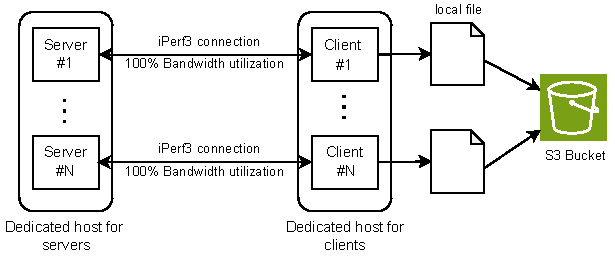
\includegraphics[width=14.5cm, height=6.25cm]{figures/netexp}
  \caption{Throughput contention experiment}
  \label{fig:netexp}
\end{figure}
\noindent
We deployed two dedicated hosts: one to host all the iPerf3 client instances and the other hosting all 
corresponding server instances.
We incrementally add client nodes that are fully utilizing their bandwidth 
through an iPerf3 connection with their paired server. Each client is continuously recording its measured 
throughput to a local log file. We implemeted a python script that computes the average of the 20 recent data 
points in the log file and append the result to a different output file. 
After each client is deployed, the script is executed across all the client nodes leveraging the distexprunner 
tool. At the end of the experiment, all the output files from the clients are uploaded to an S3 bucket 
for further analysis. \\
In the iPerf3 command executed on the clients, we set the duration (using the \texttt{-t} option) 
to 3600 seconds to ensure steady-state network performance without fluctuations caused by calling 
the command multiple times. \\
All the VMs were provisioned in the same availability zone and resided
in the same Virtual Private Cloud as mentioned in the \nameref{chapter:infra} chapter. 
